\documentclass[25pt,margin=20mm, innermargin=15mm]{tikzposter}
\usepackage[utf8]{inputenc}
\geometry{paperwidth=100cm,paperheight=100cm}
% \usetheme{Simple}
\usecolorstyle[colorPalette=Default]{Australia}
% \usebackgroundstyle{Empty}
% \usetitlestyle{Filled}
\useblockstyle{Basic}
\tikzposterlatexaffectionproofoff

\usepackage{adjustbox}

\makeatletter %To make columns scale to custom width 
\setlength{\TP@visibletextwidth}{\textwidth-2\TP@innermargin}
\setlength{\TP@visibletextheight}{\textheight-2\TP@innermargin}
\makeatother

\graphicspath{{images/}}

%%%%%%%%%%%%%%%%%%%%%%%%%%%%%%%%%%%%%%%%%%%%%%%%%%%%%%%%%%%%%%%%%%%%%%%%

\title{\parbox{\linewidth}{\centering {\bf The Challenge}: Predicting Ecosystem Collapse, Engineering Recovery}}

\author{\vspace{20pt} 
  {\begin{minipage}{9em}
    \hfill
    \centering 
    ecobuildergame.org |
  \end{minipage}
  \vspace{-20pt}}
  {\begin{minipage}{8em}
    \hfill
    \centering 
    
\includegraphics[height=2em]{Imperial_Color1.pdf}
  \end{minipage}
  \vspace{-20pt}}}
% \institute{Imperial College London}

%%%%%%%%%%%%%%%%%%%%%%%%%%%%%%%%%%%%%%%%%%%%%%%%%%%%%%%%%%%%%%%%%%%%%%%%
 
\begin{document}
 
\maketitle
 
%%%%%%%%%%%%%%%%%%%%%%%%%%%%%%%%%%%%%%%%%%%%%%%%%%%%%%%%%%%%%%%%%%%%%%%%
\block{Ecosystem Models and Data}{

	\begin{minipage}[]{0.30\linewidth}
    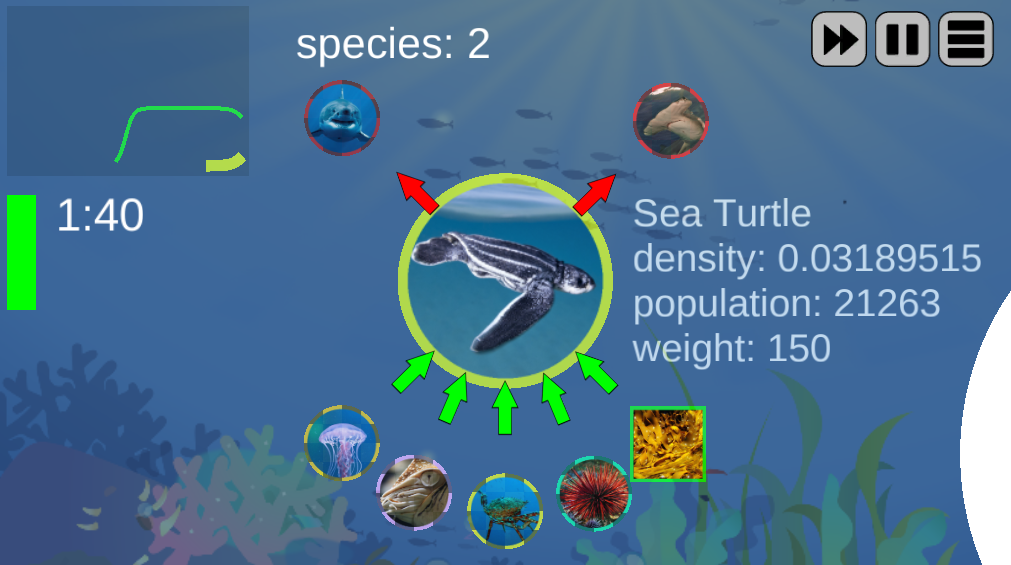
\includegraphics[width=\linewidth]{EcoBuilderA.png}
  \end{minipage}
	\hspace{.8cm}
	\begin{minipage}[]{0.38\linewidth}
			\begin{itemize} \itemsep20pt \LARGE
				\item We are building increasingly {\bf realistic 
				mathematical models of ecosystems} using {\bf theory and data on 
				species interactions} in food webs (the living ``fabric'' of 
				ecosystems). 
				\item Like the real stuff, these {model ecosystems have \bf 
				complex behavior} (Ecosystems are not a sum of their parts) --- 
				Understanding and predicting these complex behaviors 
				require {\bf computer simulations}. 
				\item The {\bf EcoBuilder game} uses one such ecosystem model. 
			\end{itemize}
		\end{minipage}
	\hspace{.5cm}
		\begin{minipage}[]{0.30\linewidth}
			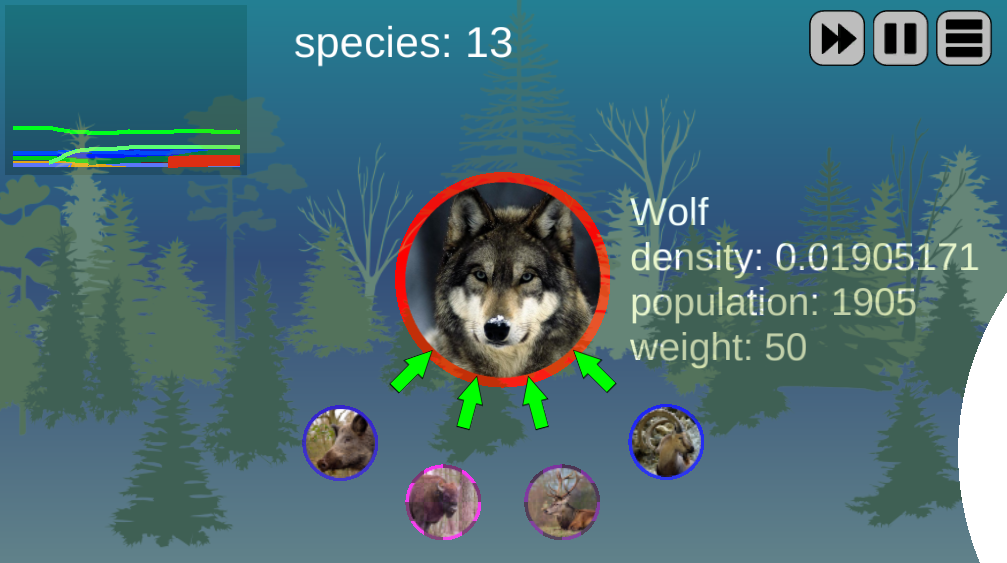
\includegraphics[width=\linewidth]{EcoBuilderT.png}
		\end{minipage}
}
 
\begin{columns}
%%%%%%%%%%%%%%%%%%%%%%%%%%%%%%%%%%%%%%%%%%%%%%%%%%%%%%%%%%%%%%%%%%%%%%%%
  \column{0.5}
    \block{How do we model species interactions?}{
	\begin{minipage}[]{0.29\linewidth}
				\begin{itemize} \itemsep20pt \large
				\item We use biomechanics and metabolic theory to generates 
				realistic ``rules'' for species interactions
			\begin{itemize} \itemsep10pt
				\item Larger-bodied species grow more slowly!
				\item Larger predators eat proportionally larger prey
				\item Increasing climatic temperature speeds up species 
				interactions
				\item Certain foraging strategies are more common  
			\end{itemize}
			\end{itemize}
			
		\end{minipage}
	\hspace{0.02\linewidth}
		\begin{minipage}[]{0.69\linewidth}\centering
			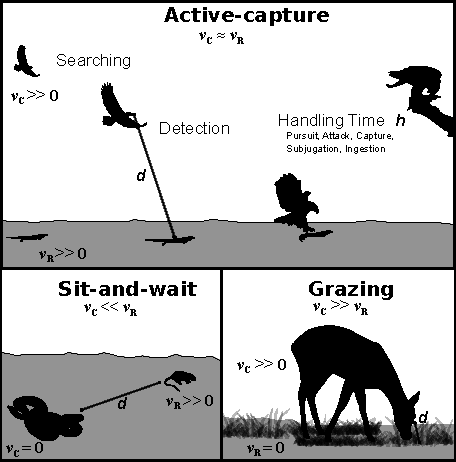
\includegraphics[width=\linewidth]{Model.pdf}
		\end{minipage}
    	}
\column{0.5}
%%%%%%%%%%%%%%%%%%%%%%%%%%%%%%%%%%%%%%%%%%%%%%%%%%%%%%%%%%%%%%%%%%%%%%%%
  \block{How do we model ecosystem collapse and recovery?}{
    
   \begin{minipage}[]{0.33\linewidth}
			\begin{itemize} \itemsep20pt \large
				\item We use species interaction rules to sequentially build or break 
				foodwebs in computer simulations
				\item \LARGE You can try this out yourself using the {\bf EcoBuilder 
				game}!
			\end{itemize}
		\end{minipage}
	\hspace{0.02\linewidth}
		\begin{minipage}[]{0.65\linewidth}\centering
			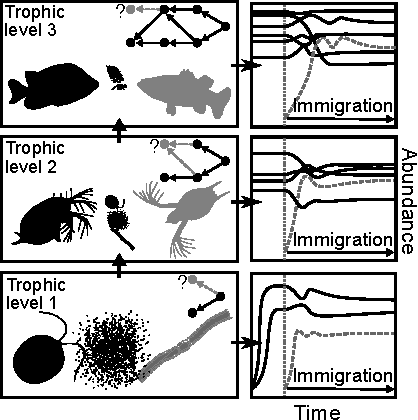
\includegraphics[width=\linewidth]{Assembly.pdf}
		\end{minipage}		
	}
\end{columns}
 
%%%%%%%%%%%%%%%%%%%%%%%%%%%%%%%%%%%%%%%%%%%%%%%%%%%%%%%%%%%%%%%%%%%%%%%%

\begin{columns}
%%%%%%%%%%%%%%%%%%%%%%%%%%%%%%%%%%%%%%%%%%%%%%%%%%%%%%%%%%%%%%%%%%%%%%%%
  \column{0.6}
\block{EcoBuilder}{\LARGE
		\begin{minipage}[]{.6\linewidth}\centering
				\begin{itemize} \itemsep20pt \LARGE
				\item EcoBuilder allows players to build an ecosystem by controlling the arrival of different types of species imto the underlying food web. 
				\item Each introduction has a ``butterfly effect'' that the player may not necessarily foresee. 
				\item This makes the game inherently challenging!
			\end{itemize}
        \end{minipage}
 	\hspace{0.07\linewidth}
 	\begin{minipage}[]{.25\linewidth}\centering
     {\it Try your hand at building an ecosystem: ecobuildergame.org!}\\
     \vspace{20pt}
     
\includegraphics[width=0.9\textwidth]{logo9.pdf}
    \end{minipage}
    }
       
   \column{0.4}
%%%%%%%%%%%%%%%%%%%%%%%%%%%%%%%%%%%%%%%%%%%%%%%%%%%%%%%%%%%%%%%%%%%%%%%%
\block{What else is going on?}{ \centering \LARGE 	
    	\begin{minipage}[]{.29\linewidth}\centering
				We are testing our models with real ecosystem data at the Silwood 
				Park Campus!
    
       \end{minipage}
		\begin{minipage}[]{.68\linewidth}\centering
         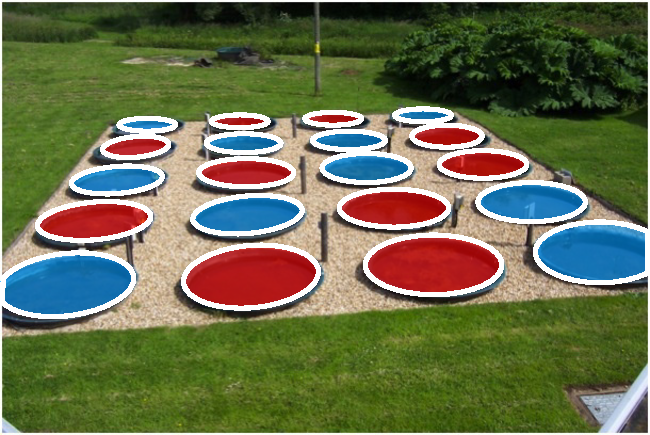
\includegraphics[width=.81\textwidth]{Mesocosms.pdf}
    \end{minipage}
	}

\end{columns}


    
 
\end{document}
